
\documentclass[a4paper,12p]{article}

% used to specify page dimentions
\usepackage[includeheadfoot,margin=2.5cm]{geometry}

% used to modify the header and the footer
\usepackage{fancyhdr}
\pagestyle{plain}

% used to change font (for this to work you need to change your engine to xelatex or luatex)
\usepackage{fontspec}
\setmainfont{Times New Roman}

% used to change paragraph spacing and line spacing
\usepackage{setspace}
\centering
\setlength{\parskip}{6pt}
\renewcommand{\baselinestretch}{1.5}

% used to set default section and subsection font sizes and spacing and style
\usepackage{titlesec}
\usepackage{sectsty}

\titleformat*{\section}{\fontsize{14pt}{12pt}\bfseries\raggedright}
\titleformat*{\subsection}{\fontsize{12pt}{6pt}\bfseries\raggedright}
\titleformat*{\subsubsection}{\fontsize{10pt}{5pt}\bfseries\raggedright}

% used to set the numbering of sections and subsections and subsubsection
\renewcommand\thesection{\arabic{section}}
\renewcommand\thesubsection{\thesection.\arabic{subsection}}
\renewcommand\thesubsubsection{}

% used to generate random text, use \lipsum[n] where n is the number of paragraphs
\usepackage{lipsum}

% for lists
\usepackage{enumitem}
\setlist{nosep}

% for images
\usepackage{graphicx}
\graphicspath{{images/}}
\usepackage[figurename=Figure]{caption}
\renewcommand{\figurename}{Figure}

\begin{document}
    % write content here
    % you will get a compilation error if this section is empty

    % add title

    % add authors
     \begin{center}
        \textbf{Raid Nasrellah TEYAR} \\
        \textbf{Oussama SALAHOUELHADJ} \\
        \textbf{Mohammed Elhadi SAOUDI} \\
    \end{center}

     \raggedright\section{Les besion fonctionnelle}

    
     \subsection{Teacher responsible of the module}
        \subsubsection{Authentication functional requirements:}
        \begin{itemize}
            \item Login
            \item retrieve password if forgotten
        \end{itemize}

        \subsubsection{Modul management functional requirements:}
        \begin{itemize}
            \item Consult modules he is responsible of
        \end{itemize}

        \subsubsection{Question bank/module management functional requirements:}
        \begin{itemize}
            \item Consult a bank of questions
        \end{itemize}

        \subsubsection{Question management functional requirements:}
        \begin{itemize}
            \item Create a question
            \item Consult a question
            \item Modify a question
            \item Delete a question
        \end{itemize}

        \subsubsection{Exam management functional requirements:}
        \begin{itemize}
            \item Create an exam
            \item Consult an exam
            \item Modify an exam
            \item Delete an exam
            \item Try an exam
            \item Confirm evaluation
            \item Consult exam analytics
            \item Publish an exam to be assigned to an exam session
            \item Export exam as pdf
        \end{itemize}

        \subsubsection{Response management functional requirements:}
        \begin{itemize}
            \item Consult list of response
            \item Consult a response
            \item Evaluate a response
        \end{itemize}

        \subsubsection{Claims management functional requirements:}
        \begin{itemize}
            \item Consult list of reclamations
            \item Consult a claim
            \item Mark a claim as done
            \item Report student
            \item Reply to a reclamation
            \item Modify reply
        \end{itemize}

        \subsubsection{Modify his own profile}


     \subsection{Teacher responsible of the td/tp}
     \subsubsection{Authentication functional requirements:}
     \begin{itemize}
         \item Login
         \item retrieve password if forgotten
     \end{itemize}

     \subsubsection{Question bank/module management functional requirements:}
     \begin{itemize}
         \item Consult a bank of questions
     \end{itemize}

     \subsubsection{Question management functional requirements:}
     \begin{itemize}
         \item Create a question
         \item Consult a question
         \item Modify a question
         \item Delete a question
     \end{itemize}

     \subsubsection{Exam management functional requirements:}
     \begin{itemize}
         \item Consult exam analytics
     \end{itemize}

     \subsubsection{Response management functional requirements:}
     \begin{itemize}
         \item Consult list of response
         \item Consult a response
         \item Evaluate a response
     \end{itemize}

     \subsubsection{Modify his own profile}

     \subsection{Student}
     \subsubsection{Authentication functional requirements:}
     \begin{itemize}
         \item Login
         \item retrieve password if forgotten
     \end{itemize}

     \subsubsection{Exams schedule management functional requirements: }
     \begin{itemize}
         \item Consult an exam
         \item Set reminder for an exam
     \end{itemize}

     \subsubsection{Pass an exam functional requirements:}
     \begin{itemize}
         \item Test requirements
         \item Check in for exam

         \item{Communicate with proctor of the exam}
         \begin{itemize}
             \item rise hand to talk to the proctor
             \item write a message to the proctor
             \item consult messages from the proctor
         \end{itemize}

         \item give feedback about his feeling in the exam
         \item leave the exam
         \item consult result of exam
     \end{itemize}

     \subsubsection{Claims functional requirements:}
     \begin{itemize}
         \item Consult a claim
         \item Claim a number of questions in an exam
     \end{itemize}

     \subsubsection{Absence functional requirements:}
     \begin{itemize}
         \item Justify an absence
         \item Consult a response
     \end{itemize}

     \subsubsection{Modify his own profile}


     \subsection{Admine: }
     \subsubsection{Authentication functional requirements:}
     \begin{itemize}
         \item Login
         \item retrieve password if forgotten
     \end{itemize}

     \subsubsection{User management functional requirements:}
     \begin{itemize}

         \item User management functional requirements
         \begin{itemize}
             \item Consult list of teachers
             \item add a teacher
             \item affect modules to a teacher
             \item modify teacher
             \item consult a teacher
             \item delete a teacher
         \end{itemize}

         \item Student management functional requirements
         \begin{itemize}
             \item consult list of students
             \item add a student
             \item modify a student
             \item consult a student
             \item delete a student
         \end{itemize}

     \end{itemize}

     \subsubsection{Module management functional requirements:}
     \begin{itemize}
         \item add a module
         \item consult a module
         \item delete a module
         \item consult list of modules
         \item modify a module
     \end{itemize}

     \subsubsection{Exam management functional requirements:}
     \begin{itemize}
         \item Create an exam session
         \item Exam's proctors management
         \begin{itemize}
             \item Assign a proctor
             \item Consult list of proctors
             \item Modify proctor
             \item Dismiss a proctor from an exam
         \end{itemize}
         \item Consult analytics of an exam
         \item Notify students
         \item Delete an exam session
         \item Absent justifications management:
         \begin{itemize}
             \item consult an absent justification
             \item consult list of absent justifications
             \item mark as done
             \item replay to report
             \item modify replay
         \end{itemize}
         \item modify an exam session
     \end{itemize}

     \subsubsection{Report management functional requirements:}
     \begin{itemize}
         \item consult list of reports
         \item consult a report
         \item mark a report as done
         \item replay to a reports
     \end{itemize}

     \subsubsection{Make configuration and database backup}
     \subsubsection{Restore configuration backup}
     \subsubsection{Restore database backup}
     \subsubsection{Modify his own profile}

     \subsection{Proctor }
     \subsubsection{Authentication functional requirements:}
     \begin{itemize}
         \item Login
         \item retrieve password if forgotten
     \end{itemize}

     \subsubsection{Session/Exam management functional requirements:}
     \begin{itemize}
         \item Control session
         \begin{itemize}
             \item start a session
             \item end exam session
             \item enable exit exam for students
             \item disable exit exam for students
             \item enable enter exam for student
             \item disable enter exam for students
             \item Confirme presence list
         \end{itemize}
         \item Communicate with student
         \begin{itemize}
             \item speak to all students
             \item speak to a student
             \item send a message to all student
             \item message one student
         \end{itemize}
         \item Kick out a particular student from the exam
         \item Monitor session live functional requirements
         \begin{itemize}
             \item proctor students
             \item pin a student
             \item proctor a student
             \begin{itemize}
                 \item write a comment about a student
                 \item end session for a particular student
             \end{itemize}
         \end{itemize}
     \end{itemize}

     \subsubsection{Modify his own profile}


     \section{DCU de chaque acteur}

     % when using images you just have to include the name of the image without the extension

    \begin{figure}[h]
        \centering
        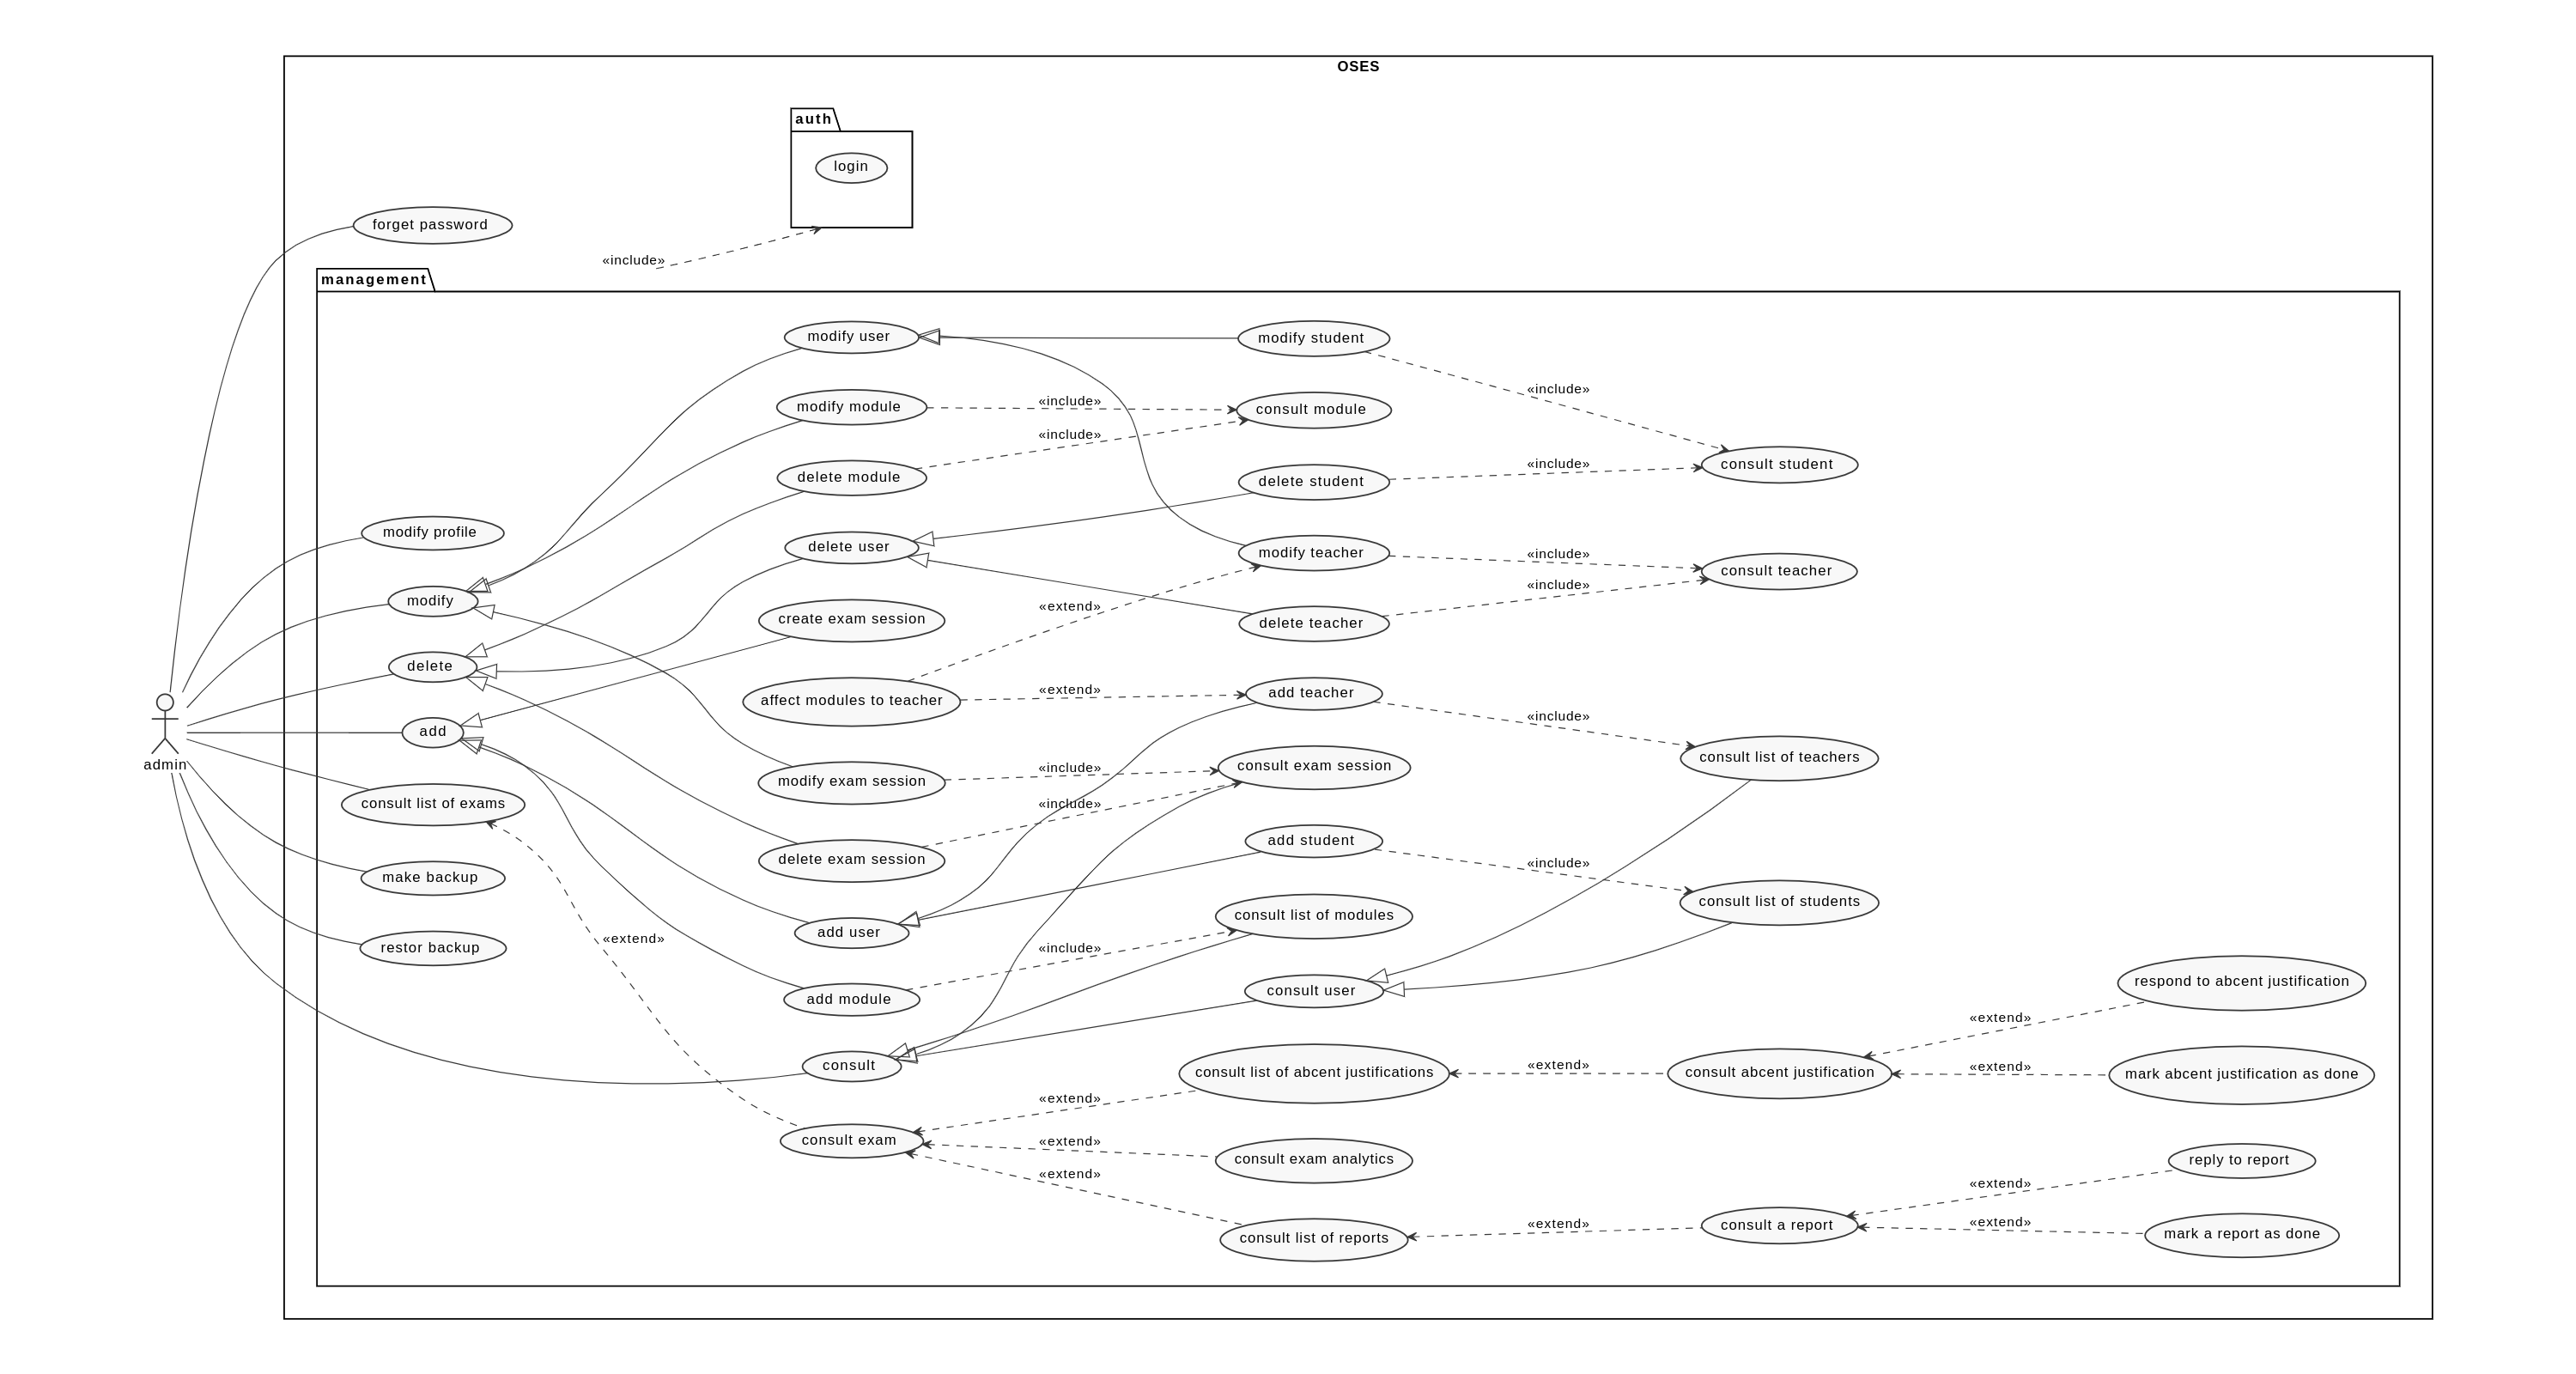
\includegraphics[width=\textwidth]{admin_UCD}
        \caption{admin use case diagram}
    \end{figure}

    \begin{figure}[h]
        \centering
        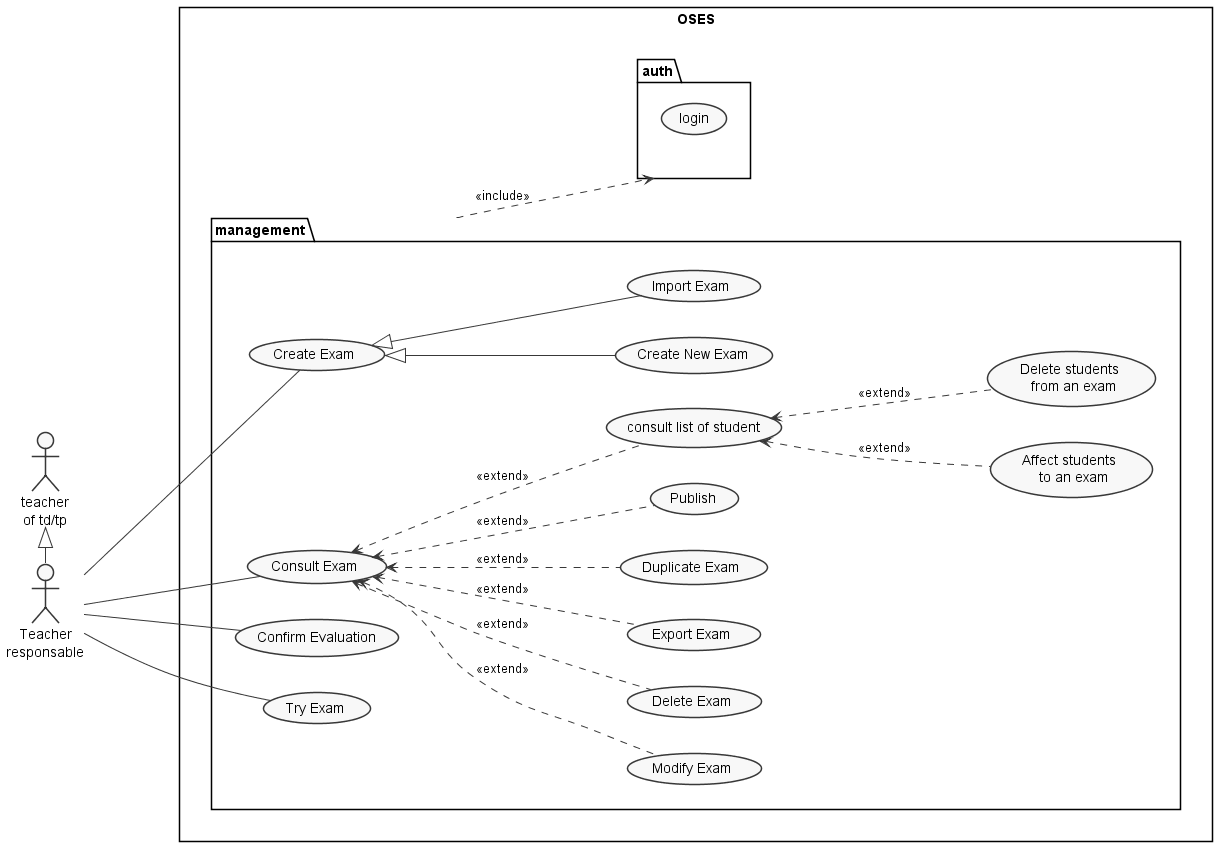
\includegraphics[width=\textwidth]{Module_Teacher}
        \caption{module teacher use case diagram}
    \end{figure}

    \begin{figure}[h]
        \centering
        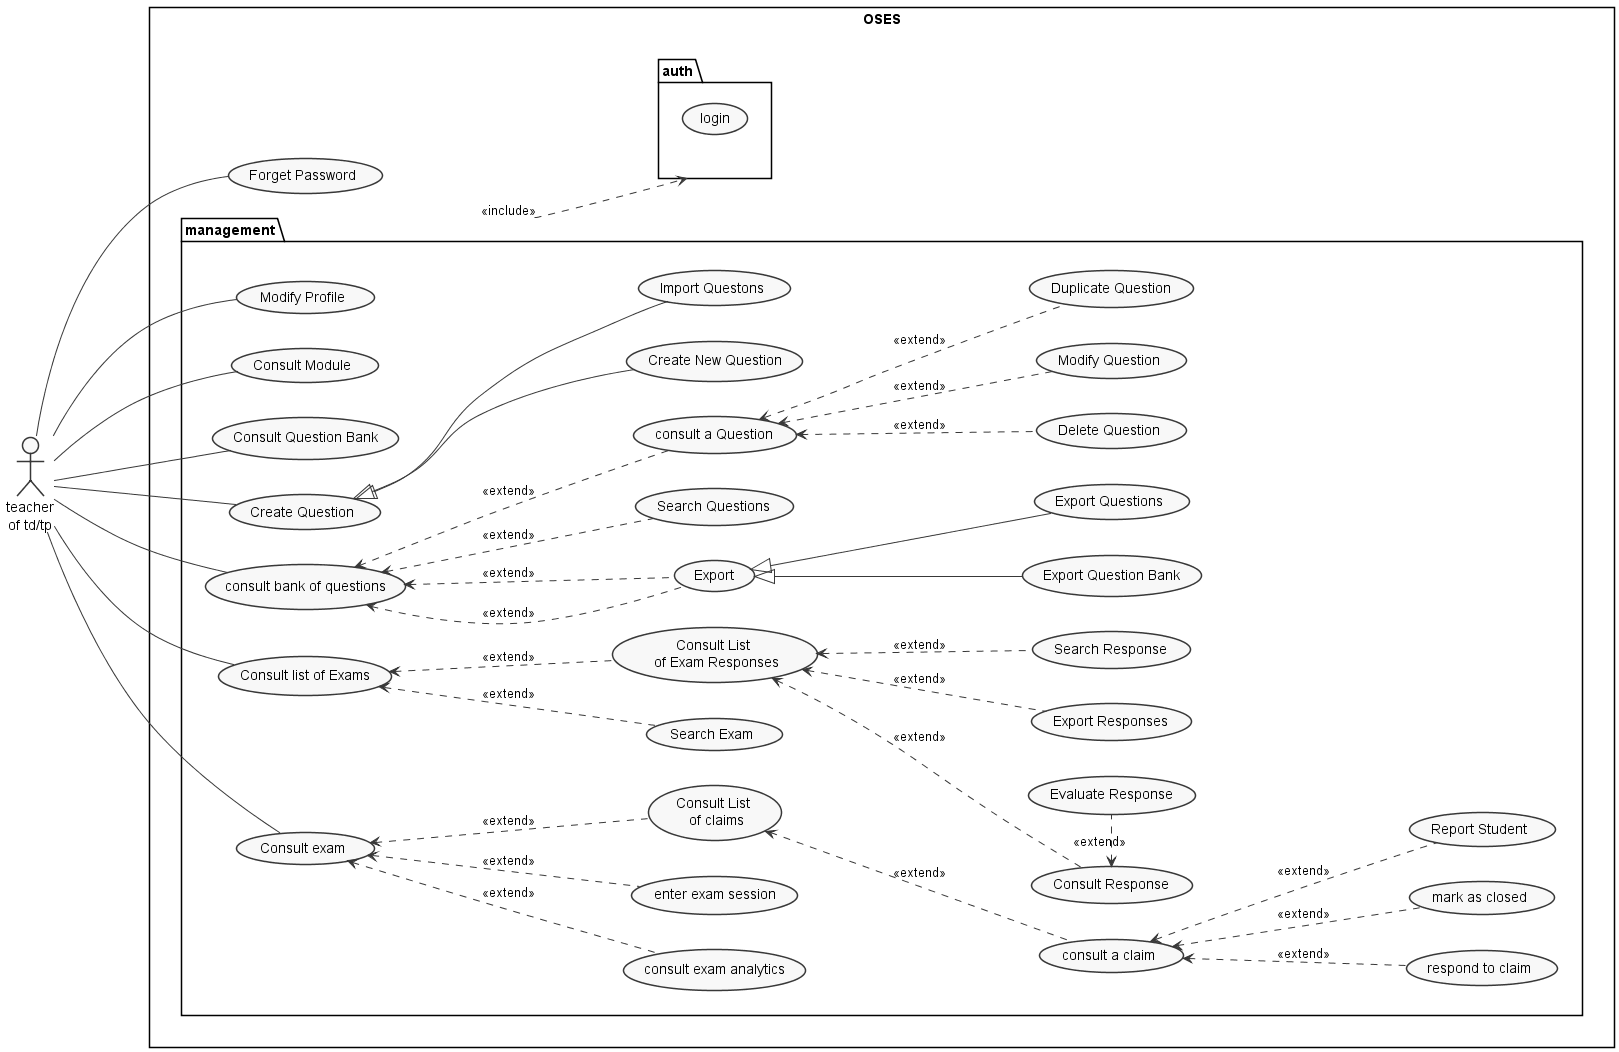
\includegraphics[width=\textwidth]{TP TD_Teacher}
        \caption{Td/Tp teacher use case diagram}
    \end{figure}

    \begin{figure}[h]
        \centering
        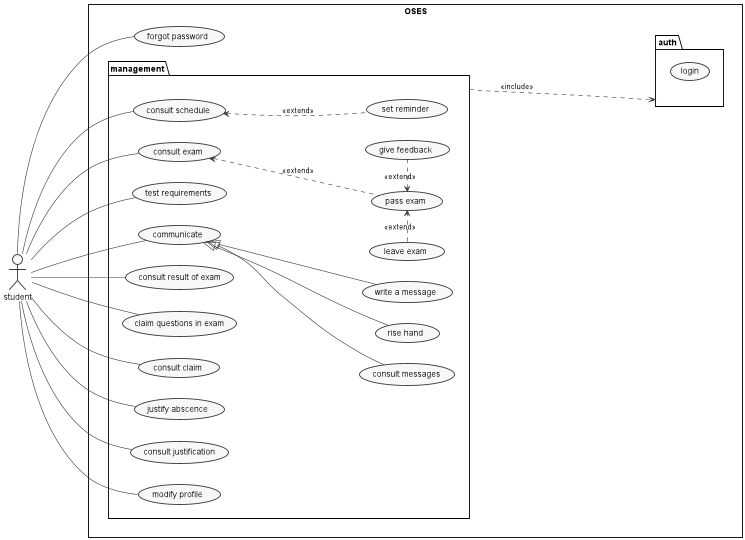
\includegraphics[width=\textwidth]{student_UCD}
        \caption{student use case diagram}
    \end{figure}

    \begin{figure}[h]
        \centering
        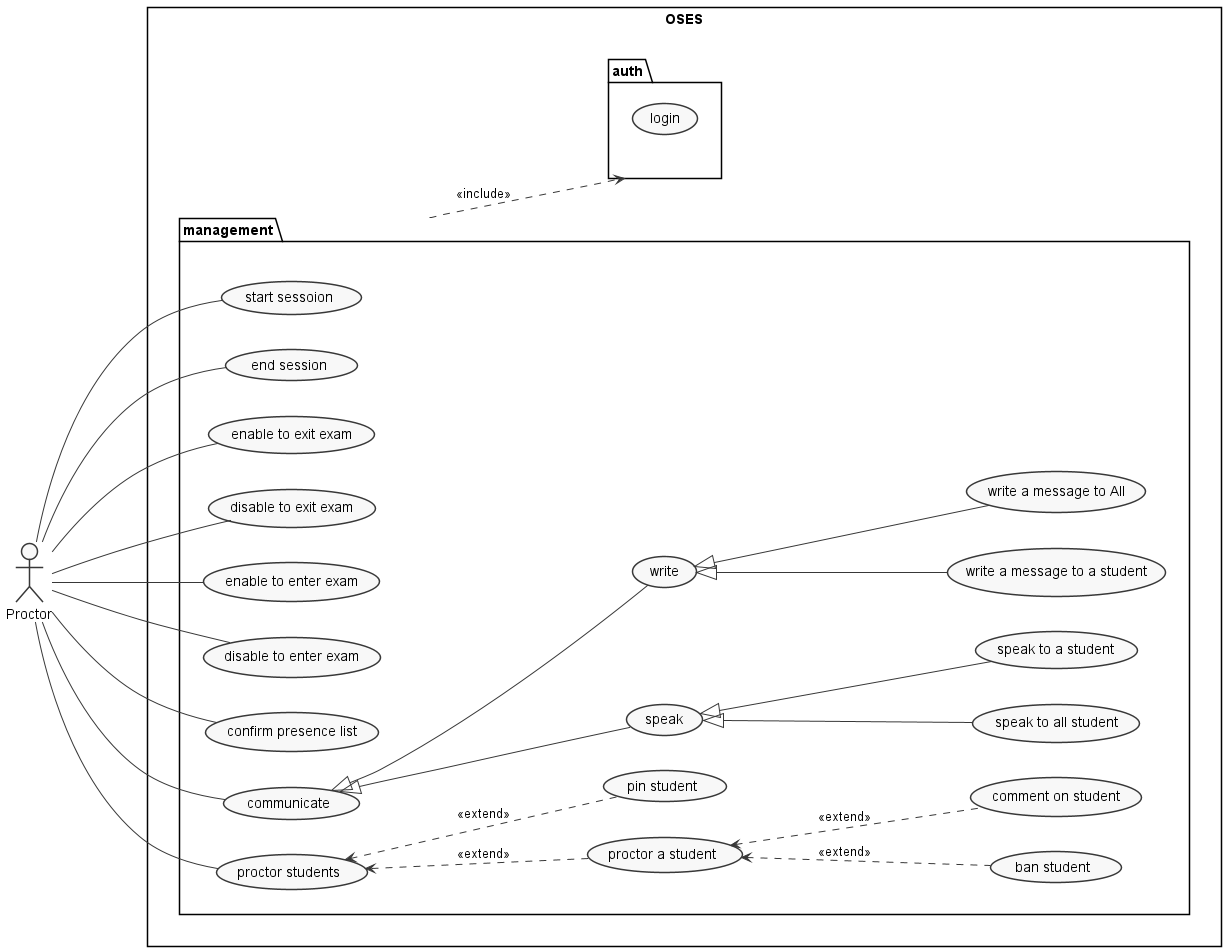
\includegraphics[width=\textwidth]{proctor_UCD}
        \caption{proctor use case diagram}
    \end{figure}

\end{document}